% =====================================================================
\chapter{Arbitrage spatial et triangulaire}
\label{ch:13}
% =====================================================================

\section{Objectifs et organisation du chapitre}

\paragraph{Objectifs.} C'est l'arbitrage que l'on voit le plus souvent promettre en ligne : acheter sur une plateforme, revendre sur une autre, ou faire tourner trois devises pour revenir avec un peu plus qu'au départ. À la fin du chapitre, vous saurez : (1) écrire les conditions exactes d'un arbitrage spatial et triangulaire avec frais ; (2) comprendre pourquoi les écarts persistent entre certaines plateformes et pas entre d'autres \citep{makarov2020} ; (3) modéliser la course à la latence et ce qu'elle implique pour un particulier \citep{budish2015} ; (4) gérer l'inventaire et les transferts entre plateformes ; (5) distinguer l'arbitrage légitime de l'arbitrage de latence interdit par les courtiers et les \emph{prop firms}.

\paragraph{Code.} \texttt{code/ch13/ch13\_spatial\_triangular.py}.

% =====================================================================
\section{Arbitrage spatial : la loi du prix unique entre plateformes}
% =====================================================================

\subsection{La condition avec frais}

Un même actif est coté sur les plateformes A et B. Notons $a_A$ le prix vendeur sur A, $b_B$ le prix acheteur sur B, et $f_A$, $f_B$ les frais taker (en fraction). Acheter une unité sur A et la vendre sur B rapporte
\[
\pi = b_B(1-f_B) - a_A(1+f_A).
\]
Il y a opportunité si $\pi>0$, soit
\[
\frac{b_B}{a_A} > \frac{1+f_A}{1-f_B} \approx 1 + f_A + f_B.
\]
L'écart relatif entre le meilleur acheteur d'un côté et le meilleur vendeur de l'autre doit dépasser la somme des frais. Entre ces bornes, les prix peuvent différer sans qu'aucun arbitrage soit possible : c'est la \emph{bande de non-arbitrage}.

\subsection{L'arbitrage avec inventaire}

Si l'on doit acheter sur A, transférer l'actif sur B puis vendre, le prix peut bouger pendant le transfert (minutes ou heures pour une cryptomonnaie, jours pour un titre) : ce n'est plus un arbitrage. En pratique, l'arbitragiste détient un inventaire sur les deux plateformes : il vend sur B l'actif qu'il possède déjà sur B et rachète simultanément sur A. Les deux ordres sont exécutés en même temps ; seul le rééquilibrage de l'inventaire nécessite un transfert, que l'on fait plus tard et plus rarement.

\paragraph{Rentabilité du rééquilibrage.} Si chaque arbitrage rapporte $e$ points de base sur un notionnel $q$ et déplace $q$ d'inventaire d'une plateforme à l'autre, un inventaire de taille $Q$ permet $Q/q$ arbitrages dans un sens avant de devoir transférer. Avec un coût de transfert fixe $K$ (frais de réseau, de retrait, temps), il faut $\frac Qq\cdot\frac{e}{10^4}\cdot q > K$, soit $Q > 10^4K/e$. Un coût de retrait de 20\,\$ et un avantage de 5 pb exigent un inventaire d'au moins $40\,000$\,\$ par côté, sans compter le coût d'opportunité du capital immobilisé et le risque de contrepartie sur chaque plateforme.

\subsection{Ce que disent les données}

\citet{makarov2020} étudient les prix du bitcoin sur de nombreuses plateformes. Ils trouvent des écarts importants et récurrents, surtout \emph{entre pays} (par exemple entre la Corée et les États-Unis), qui durent des jours ou des semaines, et des écarts beaucoup plus faibles entre plateformes d'un même pays. Les écarts entre pays s'expliquent par les contrôles des capitaux qui empêchent de rapatrier les gains : l'arbitrage existe en apparence, mais il est bloqué par une friction légale ou administrative. \textbf{Leçon :} un écart qui persiste longtemps cache presque toujours une friction (transfert impossible, risque de contrepartie, contrainte réglementaire) ; ce n'est pas de l'argent gratuit.

% =====================================================================
\section{La course à la latence}
% =====================================================================

Quand un écart est réellement exploitable sans friction, il disparaît vite, parce que plusieurs acteurs le voient au même moment et que \emph{seul le premier} est servi. \citet{budish2015} montrent que les opportunités d'arbitrage mécanique entre le future sur le S\&P~500 et l'ETF SPY n'ont pas disparu au fil des années, mais que leur durée est tombée à quelques millisecondes : la compétition s'est déplacée sur la vitesse.

\begin{codebox}[ — E1, la course à la latence]
\textbf{Protocole :} 200\,000 opportunités de gain net moyen 3 pb, de durée de vie exponentielle de moyenne 50 ms ; cinq concurrents colocalisés de latence d'environ 2 ms ; on gagne l'opportunité si notre latence est plus courte que sa durée de vie \emph{et} que celle de tous les concurrents. \textbf{Résultats :} part capturée $63{,}5\,\%$ avec 1 ms ; $3{,}0\,\%$ avec 2 ms ; $0\,\%$ dès 5 ms, et a fortiori avec 20, 100 ou 500 ms (latence typique d'un particulier passant par Internet). À l'inverse, des écarts qui durent en moyenne 5 minutes sont accessibles à $99{,}8\,\%$ avec 500 ms de latence.
\end{codebox}

\begin{figure}[h]
\centering
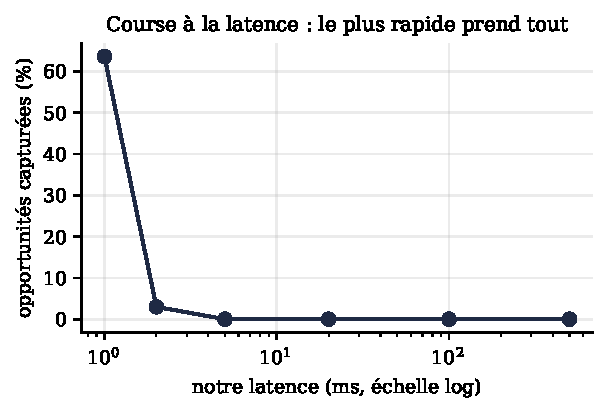
\includegraphics[width=0.6\textwidth]{ch13/course_latence.pdf}
\caption{Part des opportunités capturées en fonction de notre latence, face à des concurrents colocalisés.}
\label{c13:fig:latency}
\end{figure}

\begin{intuition}
C'est un concours où un billet tombe du ciel et où le premier qui le touche le garde. Arriver deuxième ne rapporte rien, même à un millième de seconde près. Un particulier ne gagnera jamais cette course ; il doit chercher des écarts qui ne sont pas des courses : ceux qui durent des minutes ou des jours parce qu'une friction les protège, ou ceux qui ne sont pas des arbitrages purs mais des paris de convergence (chapitre~14).
\end{intuition}

% =====================================================================
\section{Arbitrage triangulaire}
% =====================================================================

\subsection{La condition}

Trois devises EUR, USD, JPY et trois paires cotées : EUR/USD ($x$ dollars pour un euro), USD/JPY ($y$ yens pour un dollar), EUR/JPY ($z$ yens pour un euro). La cohérence impose $z = xy$. Partons d'un dollar : on achète des euros ($1/x^{ask}$ euros), avec ces euros on achète des yens ($z^{bid}/x^{ask}$ yens), avec ces yens on rachète des dollars ($z^{bid}/(x^{ask}y^{ask})$ dollars). Avec des frais $f$ à chaque étape, le cycle est profitable si
\[
\frac{z^{bid}}{x^{ask}\,y^{ask}}(1-f)^3 > 1.
\]
En points de base, si les prix milieux sont cohérents à un bruit près, le gain du cycle vaut approximativement la somme des incohérences moins trois demi-fourchettes et trois frais.

\begin{proposition}\label{c13:prop:tri}
Si l'incohérence de chacune des trois cotations est une variable normale indépendante d'écart-type $\sigma_n$ (en pb), et si chaque étape coûte une demi-fourchette $h$ et des frais $f$ (en pb), la probabilité qu'un des deux cycles soit profitable à un instant donné vaut $2\,\Prob\big(Z > \frac{3(h+f)}{\sigma_n\sqrt3}\big)$, avec $Z\sim\N(0,1)$.
\end{proposition}
\begin{proof}
Le gain du cycle direct vaut $\varepsilon_1+\varepsilon_2+\varepsilon_3 - 3(h+f)$ ; la somme des trois incohérences est normale d'écart-type $\sigma_n\sqrt3$. Le cycle inverse a pour gain l'opposé de la somme moins les mêmes coûts. Les deux événements sont disjoints (si $3(h+f)>0$) et symétriques, d'où le facteur 2.
\end{proof}

\begin{codebox}[ — E2, fréquence des opportunités triangulaires]
\textbf{Protocole :} un million d'instantanés de trois cotations. \textbf{Résultats :} demi-fourchette de 0,5 pb sans frais : $0{,}002\,\%$ des instantanés si les cotations sont cohérentes à 0,2 pb près, $38{,}6\,\%$ si elles ne le sont qu'à 1 pb près. Avec 0,5 pb de frais : 0 et $8{,}4\,\%$. Avec 2 pb de frais, niveau typique d'un particulier : $0$ et $0{,}002\,\%$. La formule de la proposition~\ref{c13:prop:tri} reproduit ces fréquences. Quand une opportunité existe, le gain moyen est inférieur à 1 pb.
\end{codebox}

Sur le marché des changes, les teneurs de marché maintiennent la cohérence des cotations croisées à une fraction de la fourchette ; les rares incohérences durent quelques millisecondes et reviennent aux plus rapides, avec des frais quasi nuls. Pour un particulier, l'arbitrage triangulaire sur le marché des changes ou sur les principales cryptomonnaies est un mirage.

% =====================================================================
\section{L'arbitrage de latence : une ligne rouge}
% =====================================================================

Une variante très répandue chez les particuliers consiste à exploiter le retard du flux de prix d'un courtier de CFD ou d'une \emph{prop firm} par rapport à un flux plus rapide : quand le prix \og vrai\fg{} bouge, on achète chez le courtier au prix encore ancien. Ce n'est pas un arbitrage entre deux marchés, c'est l'exploitation d'une faiblesse technique du fournisseur, qui en supporte directement la perte. Les conditions générales des courtiers et des \emph{prop firms} l'interdisent explicitement ; elles interdisent aussi la couverture croisée entre comptes \citep{nexusfi}. Les conséquences vont de l'annulation des gains à la fermeture du compte. Ce cours ne traite pas de ces pratiques, sauf pour vous dire de ne pas les déployer, en particulier sur vos comptes de \emph{prop firms}.

% =====================================================================
\section{Ce que la théorie apporte, et ses limites}
% =====================================================================

\paragraph{Apports.} Des conditions exactes avec frais, une explication de la persistance de certains écarts (frictions), un modèle simple de la course à la latence, et un critère d'inventaire pour l'arbitrage entre plateformes.

\paragraph{Limites.} Les opportunités réelles dépendent de la profondeur du carnet (on ne peut souvent exécuter qu'une petite quantité au meilleur prix), du risque de contrepartie des plateformes, des délais et des coûts de transfert, et de contraintes réglementaires et fiscales que les modèles ignorent.

% =====================================================================
\section{Fiche à recopier au tableau blanc}
% =====================================================================

\begin{whiteboard}
\begin{itemize}[leftmargin=1.2em]
\item \textbf{Spatial :} opportunité si $b_B/a_A > (1+f_A)/(1-f_B)\approx1+f_A+f_B$.
\item \textbf{Inventaire :} rééquilibrage rentable si $Q > 10^4K/e$ ($K$ coût de transfert, $e$ avantage en pb).
\item \textbf{Écart persistant :} chercher la friction (contrôle des capitaux, transfert, contrepartie).
\item \textbf{Latence :} le premier prend tout ; durée de vie en millisecondes $\Rightarrow$ inaccessible au particulier.
\item \textbf{Triangulaire :} profitable si $z^{bid}(1-f)^3/(x^{ask}y^{ask}) > 1$ ; probabilité $2\Prob(Z > 3(h+f)/(\sigma_n\sqrt3))$.
\item \textbf{Ligne rouge :} arbitrage de latence contre un courtier ou une \emph{prop firm} : interdit.
\end{itemize}
\end{whiteboard}

% =====================================================================
\section{Exercices}
% =====================================================================

\begin{exercise}
Le BTC est coté $64\,000$ à la vente sur A et $64\,050$ à l'achat sur B ; frais taker de 0,10\,\% sur A et 0,06\,\% sur B. Y a-t-il une opportunité ? Quel écart minimal faudrait-il ?
\end{exercise}

\begin{exercise}
Démontrez l'approximation $(1+f_A)/(1-f_B)\approx 1+f_A+f_B$ par un développement limité à l'ordre 1, et estimez l'erreur pour $f_A = f_B = 0{,}1\,\%$.
\end{exercise}

\begin{exercise}
Un inventaire de $20\,000$\,\$ par côté, un avantage moyen de 4 pb par arbitrage de $1\,000$\,\$, un coût de rééquilibrage de 15\,\$. Le rééquilibrage est-il rentable ? Combien d'arbitrages faut-il entre deux rééquilibrages ?
\end{exercise}

\begin{exercise}[à coder]
Dans E1, donnez aux opportunités une durée de vie qui dépend de leur taille (les grands écarts disparaissent plus vite). Comment évolue le gain moyen d'un acteur lent ?
\end{exercise}

% =====================================================================
\section{Pour aller plus loin}
% =====================================================================

\begin{toread}
\begin{itemize}[leftmargin=1.2em]
\item \citet{makarov2020} : les sections sur les écarts entre pays et sur le rôle des contrôles de capitaux.
\item \citet{budish2015} : la section empirique sur la durée des opportunités ES/SPY et l'argument de la course aux armements.
\item \citet{harris2003} : les chapitres consacrés aux arbitragistes et à la fragmentation des marchés.
\end{itemize}
\end{toread}

\section{Scripts du chapitre}
\noindent\texttt{code/ch13/ch13\_spatial\_triangular.py} : E1 (figure~\ref{c13:fig:latency}), E2.
